\chapter{Resoconto attività di verifica}\label{resoconto-attivita-di-verifica}

\section{Indici Gulpease}

\begin{center}
    \begin{xltabular}{\linewidth}{|l|l|l|}
    \hline
    \rowcolor[gray]{0.9}
    \textbf{Documento} & \textbf{Valore} & \textbf{Esito} \\
    \hline
     Analisi dei requisiti & 76 & Accettabile \\
     Piano di qualifica & 75 & Accettabile \\
     Piano di progetto & 73 & Accettabile \\
     Norme di progetto & 77 & Accettabile \\
     Verbali (media) & 73 & Accettabile \\ 
    \hline

    \end{xltabular}
\end{center}

\begin{figure}
    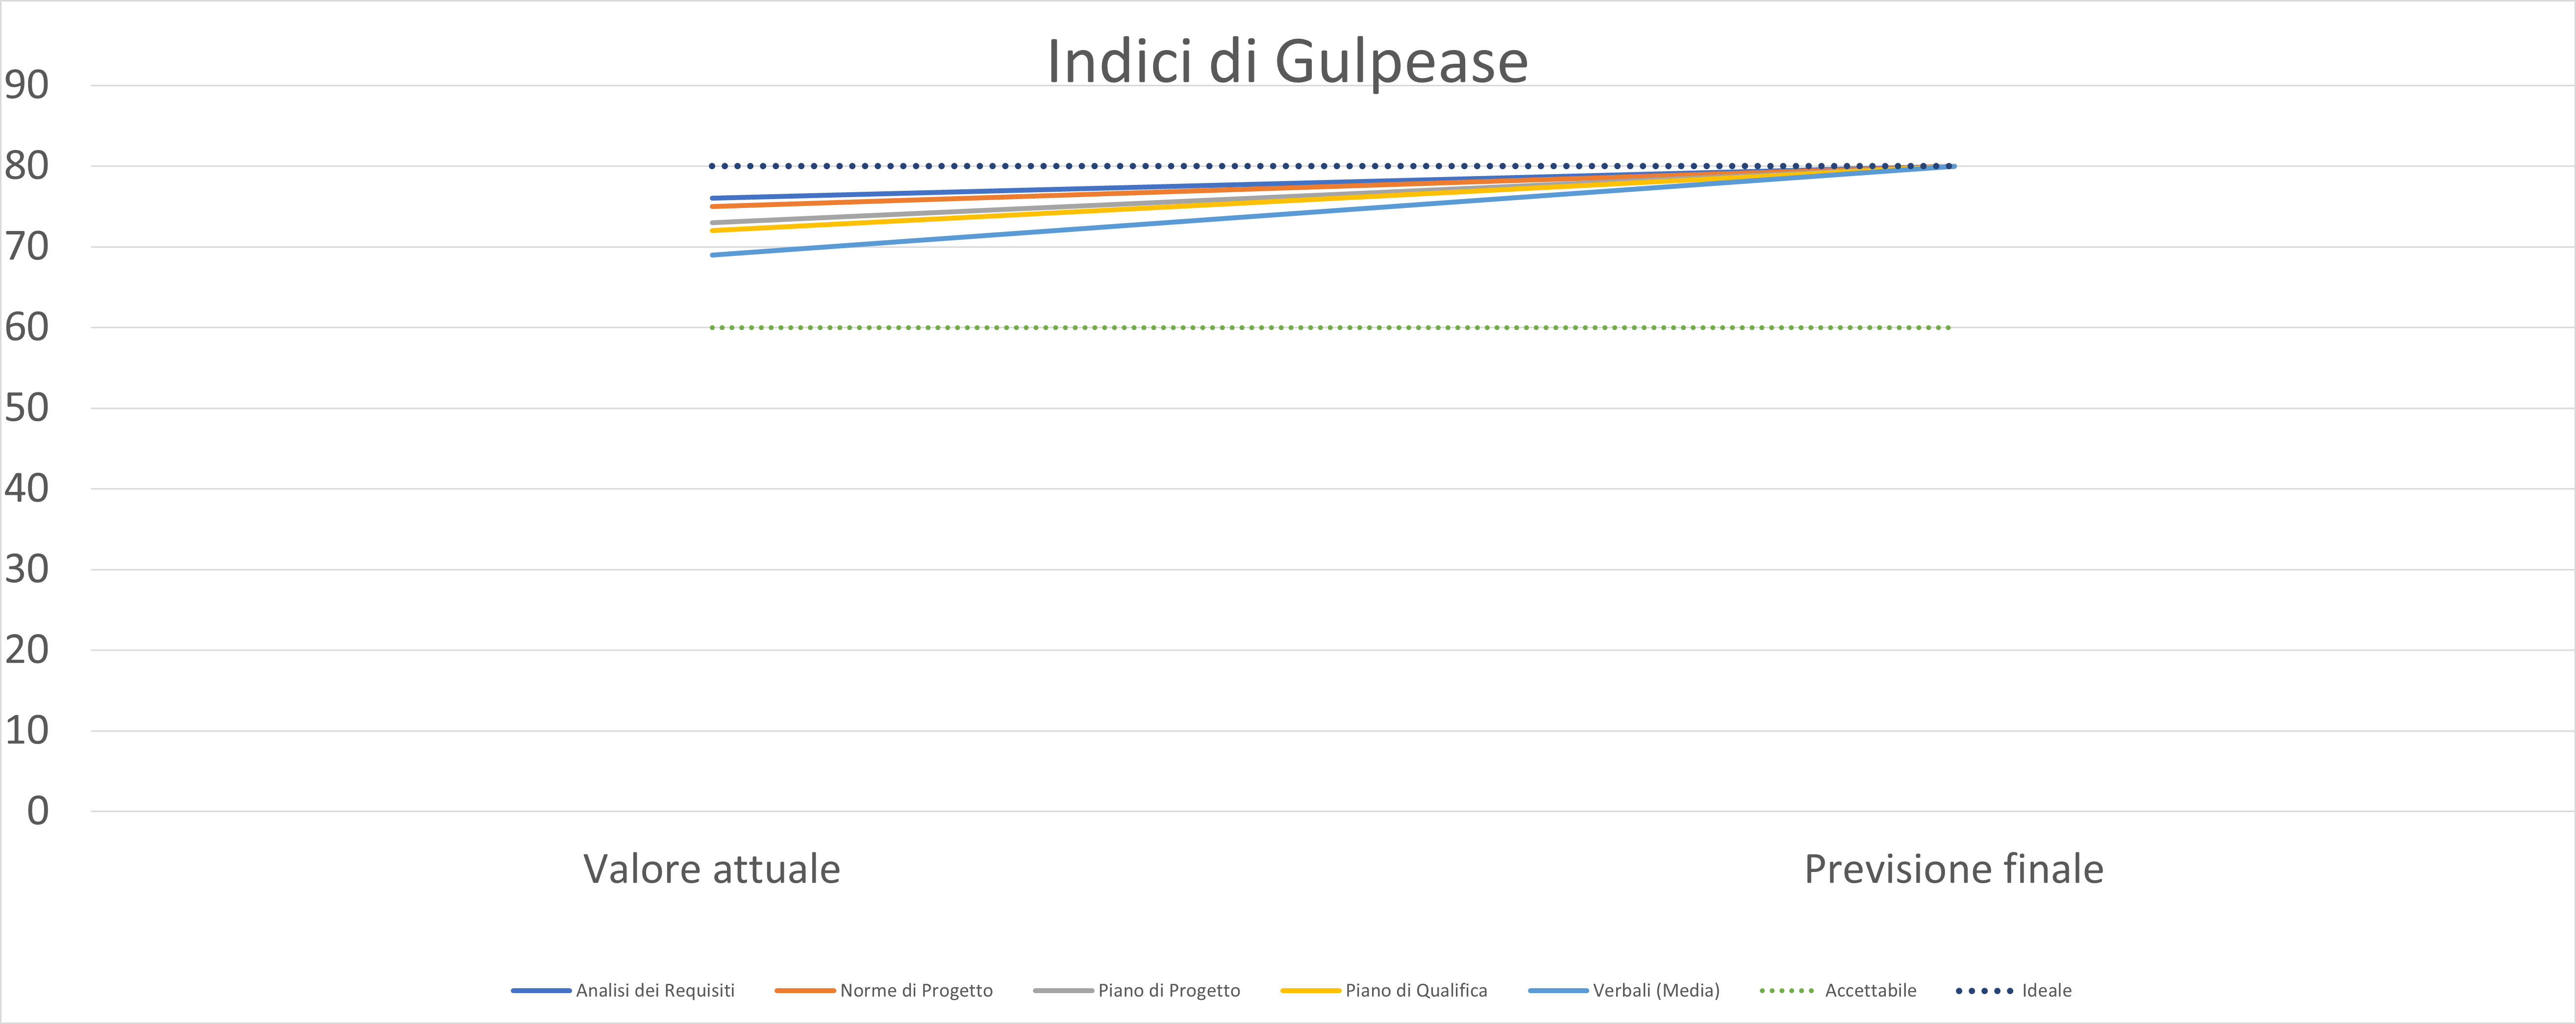
\includegraphics[width=\linewidth]{contenuti/img/gulpease.png}
    \caption{Indice Gulpease documentazione}
  \end{figure}

\section{Errori grammaticali}

\begin{center}
    \begin{xltabular}{\linewidth}{|l|l|l|}
    \hline
    \rowcolor[gray]{0.9}
    \textbf{Documento} & \textbf{Valore} & \textbf{Esito} \\
    \hline
     Analisi dei requisiti & 0 & Ideale \\
     Piano di qualifica & 0 & Ideale \\
     Piano di progetto & 0 & Ideale \\
     Norme di progetto & 0 & Ideale \\
     Verbali (media) & 0 & Ideale \\ 
    \hline

    \end{xltabular}
\end{center}